
The given equations result in the matrix equation
In vector form:
\begin{align}
\myvec{6 & 0 & -1 \\
0 & 3 & -1 \\
1 & 1 & 1 
}\myvec{A \\ B \\ C} &= \myvec{0\\0\\180}
\end{align}
whcih can be solved as
\begin{align}
\myvec{6 & 0 & -1 & 0 \\
0 & 3 & -1 & 0 \\
1 & 1 & 1 & 180
}
&\xleftrightarrow[]{R_1 \leftarrow \frac{R_1}{6}}
\myvec{1 & 0 & \frac{-1}{6} & 0 \\
0 & 3 & -1 & 0 \\
1 & 1 & 1 & 180
}\\
\xleftrightarrow[]{R_3 \leftarrow R_3 - R_1}
\myvec{1 & 0 & \frac{-1}{6} & 0\\
0 & 3 & -1 & 0 \\
0 & 1 & \frac{7}{6} & 180}
&\xleftrightarrow[]{R_2 \leftarrow \frac{R_2}{3}}
\myvec{1 & 0 & -\frac{1}{6} & 0 \\
0 & 1 & -\frac{1}{3} & 0 \\
0 & 1 & \frac{7}{6} & 180
}\\
\xleftrightarrow[]{R_3 \leftarrow \ R_3-R_2}
\myvec{1 & 0 & -\frac{1}{6} &  0 \\
0 & 1 & -\frac{1}{3} & 0 \\ 
0 & 0 & \frac{3}{2} & 180
}
&\xleftrightarrow[]{R_3 \leftarrow \ \frac{2R_3}{3}}
\myvec{1 & 0 & -\frac{1}{6} &  0 \\
0 & 1 & -\frac{1}{3} & 0 \\ 
0 & 0 & 1 & 120
}\\ 
\xleftrightarrow[R_2 \leftarrow \ R_2+ \frac{R_3}{3}]{R_1 \leftarrow \ R_1 + \frac{R_3}{6}}
\myvec{1 & 0 & 1 &  20 \\
0 & 1 & 0 & 40 \\ 
0 & 0 & 1 & 120
}& 
\end{align}

\begin{align}
\therefore \angle C = 120\degree \ \angle A = 20\degree \ \angle B &= 40\degree 
\end{align}

%\item \begin{figure}[!h]
%\centering
%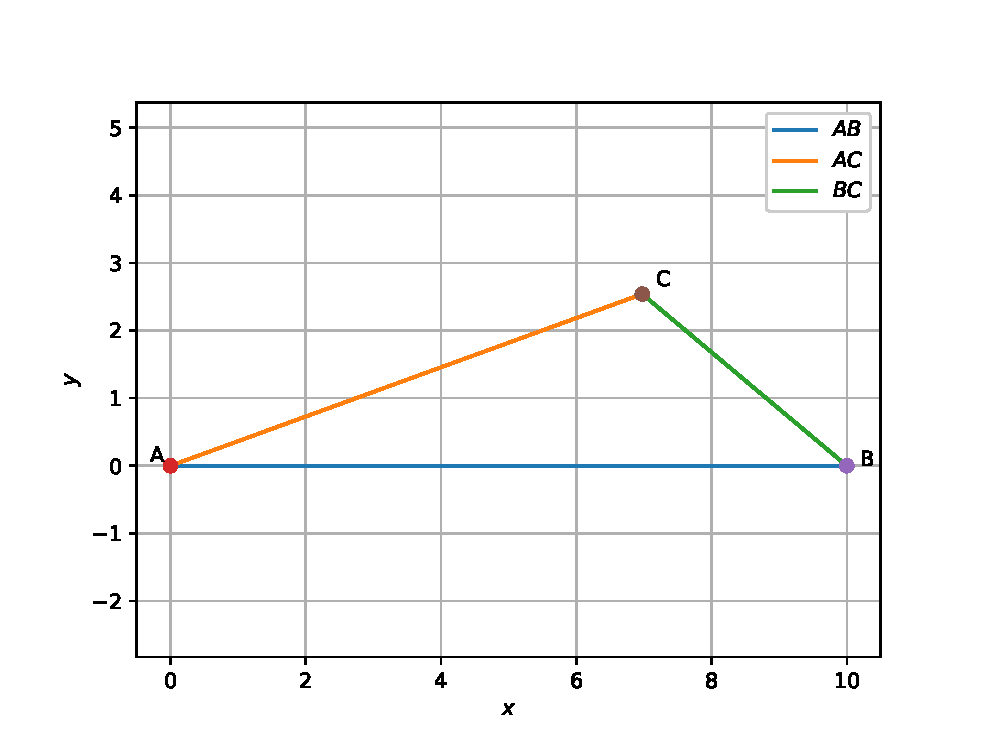
\includegraphics[width=\columnwidth]{./figs/triangle_ex/triangle_linearalg.eps}
%\caption{Triangle generated using python}
%\label{fig:triangle2_triangle_ex}
%\end{figure} 
%
%The  following Python code generates Fig. \ref{fig:triangle2_triangle_ex}
%
%\begin{lstlisting}
%codes/triangle_ex/triangle_linearalg.py
%\end{lstlisting}
%
%\end{enumerate}
%
